\documentclass[../../Cours_M1.tex]{subfiles}

\newcommand{\nomTD}{TP2 : Réalisation d'une PLL à éléments discrets}
\renewcommand{\nomentete}{UE431 - \nomTD}
\renewcommand{\auteur}{Aymeric Arnould, Tom Colinot}

\title{\nomTD}
\author{\auteur}

\renewcommand{\thesection}{\Roman{section}}

\begin{document}

\maketitle

\begin{center}
\textbf{A. Préparation}
\end{center}

\section{Étude de la boucle à verrouillage de phase}

\subsection{Mise sous forme de schéma blocs}

On donne le schéma de principe d'une PLL \footnote{Phase Locked Loop : Boucle à verrouillage de phase} :

\begin{figure}[h!]
\centering
\begin{tikzpicture}
\sbEntree{E}

\sbBloc[4]{comp}{Comparateur de phase}{E}
\sbRelier[$v_e(t)$]{E}{comp}

\sbBloc[4]{pb}{Filtre passe-bas}{comp}
\sbRelier[$v_1(t)$]{comp}{pb}

\sbBloc[4]{sys}{VCO}{pb}
\sbRelier[$v_2(t)$]{pb}{sys}

\sbSortie[4]{S}{sys}
\sbRelier[$v_s(t)$]{sys}{S}

\sbRenvoi{sys-S}{comp}{}

\end{tikzpicture}
\caption{Schéma de principe d'une PLL}
\end{figure}

On s'intéresse aux phases $\phi_e(t)$ et $\phi_s(t)$ comme grandeurs d'entrée et de sortie.
\[\omega_s(t) = \frac{d\phi_s(t)}{dt} \]

On a donc dans l'espace de Laplace :
\[ \Omega_s(p) = p\Phi_s(p) \]

Le comparateur de phase est linéaire de gain $K_1$ :
\[ v_1(t) = K_1[\phi_e(t)-\phi_s(t)] \]
\[V_1(p) = K_1[\Phi_e(t)-\Phi_s(t)] \]

On utilise un VCO \footnote{Oscillateur contrôlé en tension} centré sur une fréquence nulle :
\[f_s(t) = K_3v_2(t) \]
\[\Phi_s(p) = \frac{2\pi}{p} f_s(t) = \frac{2\pi}{p}K_3 v_2(t)\]

On a donc le schéma-blocs suivant :
\begin{figure}[h!]
\centering
\begin{tikzpicture}
\sbEntree{E}
\sbComp{comp}{E}
\sbRelier[$\Phi_e(p)$]{E}{comp}

\sbBloc[4]{phcomp}{$K_1$}{comp}
\sbRelier{comp}{phcomp}

\sbBloc[4]{H}{$H(p)$}{phcomp}
\sbRelier[$V_1(p)$]{phcomp}{H}

\sbBloc[4]{sys}{$\frac{2\pi K_3}{p}$}{H}
\sbRelier[$V_2(p)$]{H}{sys}

\sbSortie[4]{S}{sys}
\sbRelier[$\Phi_s(p)$]{sys}{S}
\sbRenvoi{sys-S}{comp}{}
\end{tikzpicture}
\caption{Schéma blocs}
\end{figure}

En utilisant les fréquences comme grandeurs d'entrée et de sortie, on garde une structure telle que le comparateur soit toujours relatif au phases et non aux fréquences :

\begin{figure}[h!]
\centering
\begin{tikzpicture}
\sbEntree{E}

\sbBloc[4]{int}{$\frac{2\pi}{p}$}{E}
\sbRelier[$F_e(p)$]{E}{int}

\sbComp{comp}{int}
\sbRelier[$\Phi_e(p)$]{int}{comp}

\sbBloc[4]{phcomp}{$K_1$}{comp}
\sbRelier{comp}{phcomp}

\sbBloc[4]{H}{$H(p)$}{phcomp}
\sbRelier[$V_1(p)$]{phcomp}{H}

\sbBloc[4]{sys}{$K_3$}{H}
\sbRelier[$V_2(p)$]{H}{sys}

\sbSortie[4]{S}{sys}
\sbRelier[$F_s(p)$]{sys}{S}

\sbDecaleNoeudy[4]{S}{R}
\sbBlocr[12]{intr}{$\frac{2\pi}{p}$}{R}
\sbRelieryx{sys-S}{intr}
\sbRelierxy[$\Phi_s(p)$]{intr}{comp}

\end{tikzpicture}
\caption{Schéma blocs}
\end{figure}

\subsection{Etude complète de la boucle à verrouillage de phase}

On suppose que le filtre est un passe-bas d'ordre 1 :
\[H(p) = \frac{1}{1+\tau p} \]

\subsubsection*{I.2.1 Etude de la stabilité}

La fonction de transfert en boucle ouverte de la PLL en phase est :
\[T(p) = \frac{2\pi K_1 K_3}{p(1+\tau p)} \]

On a donc en boucle fermée en phase :
\[F_{BF}(p) = \frac{T(p)}{1+T(p)} = \frac{1}{\frac{\tau}{K_1K_32\pi}p^2+\frac{1}{K_1K_32\pi}p+1}\]

\subsubsection*{I.2.2 Etude du régime établi}

\begin{multicols}{2}
Vis-à-vis de la phase,
\[ \epsilon_{\Phi}(p) = \frac{1}{1+\frac{2\pi K_1 K_3}{p(1+\tau p)}} \Phi(p) \]

Pour une entrée en phase de type rampe :
\begin{align*}
\lim_{t\rightarrow\infty} \epsilon(t) & = \lim_{p\rightarrow 0} pE(p) \\
& = \lim_{p\rightarrow 0} p \frac{\Phi_0}{p^2} \frac{1}{1+\frac{2\pi K_1 K_3}{p(1+\tau p)}} \\
& = \lim_{p\rightarrow 0} \Phi_0 \frac{1}{p+\frac{2\pi K_1 K_3}{1+\tau p}} \\
\lim_{t\rightarrow\infty} \epsilon(t) & = \frac{\Phi_0}{2\pi K_1 K_3}
\end{align*}


Vis-à-vis de la fréquence :
\[ \epsilon_F(p) = \frac{\frac{2\pi}{p}}{1+\frac{2\pi K_1 K_3}{p(1+\tau p)}} F(p) \]

Pour une entrée en fréquence en échelon :
\begin{align*}
\lim_{t\rightarrow\infty} \epsilon(t) & = \lim_{p\rightarrow 0} pE(p) \\
& = \lim_{p\rightarrow 0} p \frac{F_0}{p} \frac{\frac{2\pi}{p}}{1+\frac{2\pi K_1 K_3}{p(1+\tau p)}} \\
& = \lim_{p\rightarrow 0} F_0 \frac{2\pi}{p+\frac{2\pi K_1 K_3}{1+\tau p}} \\
\lim_{t\rightarrow\infty} \epsilon(t) & = \frac{F_0}{K_1K_3}
\end{align*}
\end{multicols}

La réponse à un échelon en fréquence correspond à la réponse à une rampe en phase.

En effet, $f(t) = \frac{1}{2\pi} \frac{d\phi(t)}{dt}$ donc $F(p) = \frac{p \Phi(p)}{2\pi}$.

Imposer un échelon de fréquence $F(p) = \frac{F_0}{p}$ revient en phase à $\Phi(p) = \frac{2\pi F_0}{p^2}$ (rampe).\\

\subsubsection*{I.2.3 Etude du comportement dynamique (régime transitoire)}

On donne $|K_1| = 5/\pi$ V/rad.s et $|K_3| = 20,7$ kHz/V. On a $\tau = \frac{1}{2\pi f}$ avec $f = 1 $ puis 5 kHz.

\[F_{BF}(p) = \frac{1}{\frac{p^2}{\omega_0^2}+\frac{2m}{\omega_0}p +1}\]

On a donc
\[ \omega_0 = \sqrt{\frac{K_1K_3 2\pi}{\tau}}  \quad \et \quad
m = \frac{1}{2\sqrt{\tau K_1 K_3 2 \pi}} \]

\begin{center}
\begin{tabular}{|c|c|c|}
\hline
$f_c$ (kHz) & $\omega_0$ (rad/s) & m \\
\hline
5 & 60642 & 0,195 \\
\hline
1 & 36064 & 0,087 \\
\hline
\end{tabular}
\end{center}

\section{Étude des différents blocs}

\subsection{Le comparateur de phase OU EXCLUSIF}

On écrit la table de vérité du OU EXCLUSIF :
\begin{center}
\begin{tabular}{|c|c|c|}
\hline
$a$ & $b$ & $a\oplus b$ \\
\hline
0 & 0 & 0 \\
\hline
0 & 1 & 1 \\
\hline
1 & 0 & 1 \\
\hline
1 & 1 & 0 \\
\hline
\end{tabular}
\end{center}

On calcule la valeur moyenne du signal de sortie du OU EXCLUSIF :
\[<v_1(t)>_T = \frac{\phi}{\pi} V_{DD}\]

Or, on a aussi :
\[<v_1(t)>_T = K_1 <\phi_e(t)-\phi_s(t)>\]

Ainsi, on a $K_1 = \frac{\phi}{\pi}V_{DD}$.

À la borne - de l'AO \footnote{Amplificateur Opérationnel}, on a grâce au théorème de Millman :
\[ V^-=\frac{V_A+V_B}{2} \]

À la borne + de l'AO, on a un diviseur de tension :
\[ V^+=\frac{1}{1+jR_0C_0\omega}V_A\]

Avec un AO parfait, $V^+ = V^-$. Cela conduit à
\[ \frac{V_B}{V_A} = \frac{1-jR_0C_0\omega}{1+jR_0C_0\omega} \]

Ainsi, on a un gain unitaire : ce montage est un déphaseur, et
\[ \arg(\frac{V_B}{V_A}) = -2\arctan(R_0C_0\omega) \]

Il est donc possible de créer à partir de $V_A(t)$, un signal $V_B(t)$  avec un déphasage variant entre 0 et -180 degrés.

Les deux AO en sortie de montage permettent de donner une petite impédance de sortie au montage, dans le but de placer d'autres circuits en sortie sans influencer le fonctionnement du déphaseur.

\subsection{Le filtre}

On utilise un pont diviseur de tension $R_1,C_1$ série aux bornes e $C_1$. La fonction de transfert correspondante est :
\[H(p) = \frac{1}{1+jR_1C_1\omega} \]

Le diagramme de Bode du filtre passe-bas est le suivant :

En réalité, le comparateur de phase fournit une tension comportant un terme fonction de la différence des phases ET un terme fonction de la somme des phases (Haute fréquence). Le filtre passe-bas permet de supprimer le second pour ne garder que le terme correspondant à la différence des phases.

Avec  $R_1 = 15 k\Omega$, comme $R_1 = \frac{1}{2\pi f C_1}$, on a
\begin{center}
\begin{tabular}{|c|c|}
\hline
$f_c$ (kHz) & $C_1$ (nF) \\
\hline
5 & 2,1 \\
\hline
1 & 11 \\
\hline
\end{tabular}
\end{center}

\subsection{L'oscillateur contrôlé en tension}

\subsubsection{L'oscillateur d'Abraham et Bloch}

\textbf{II.3.1.1 Analyse qualitative} \\

\noindent Lorsque les capacités $C_1$ et $C_2$ ne sont pas connectées :

Maille passant par collecteur/émetteur de $T_i$ puis par $R_{Ci}$ :
\begin{multicols}{2}
\[V_{CC} = V_{CE1} + R_{C1}I_{C1} \]
donc
\[I_{C1} = \frac{V_{CC}-V_{CE1}}{R_{C1}}\]

\[V_{CC} = V_{CE2} + R_{C2}I_{C2} \]
donc
\[I_{C2} = \frac{V_{CC}-V_{CE2}}{R_{C2}}\]
\end{multicols}

Maille passant par base/émetteur de $T_i$ puis par $R_{Cj}$ :
\begin{multicols}{2}
\[V_{CC} = V_{BE1} + R_{B2}I_{B1} \]
donc
\[I_{B1} = \frac{V_{CC}-V_{BE1}}{R_{B2}}\]

\[V_{CC} = V_{BE2} + R_{B1}I_{B2} \]
donc
\[I_{B2} = \frac{V_{CC}-V_{BE2}}{R_{B1}}\]
\end{multicols}

Lorsque les transistors fonctionnent en saturation, on a pour les deux transistors $V_{CE} = V_{CE}^{sat} = 0$ et $V_{BE} = V_{\delta}$. De plus, $I_C = \beta I_B$ donc on doit avoir :

\begin{align*}
\frac{V_{CC}}{R_{C1}} & = \beta \frac{V_{CC}-V_{\delta}}{R_{B2}} \\
\frac{V_{CC}}{R_{C2}} & = \beta \frac{V_{CC}-V_{\delta}}{R_{B1}}
\end{align*}

\noindent On s'intéresse au schéma complet. Les condensateurs sont initialement déchargés et on met le circuit sous tension. Les condensateurs $C_1,C_2$ se chargent via les résistances $R_1,R_2$.

On suppose que $T_2$ sature avant $T_1$.

\begin{itemize}
%\item $T_2$ est saturé donc $V_{C2}= V_{CE2} = 0$V. On a alors $u_2 = -V_{BE1}$.
%
%La base de $T_2$ est portée à $V_{BE2} = V_{\delta}=0,7$V, donc $V_{C1} = u_1 + 0,7$.
%
%$T_1$ est bloqué donc sa base $V_{BE1} < V_{\delta}$. Les condensateurs étant presque chargés, on a $V_{C1} \approx V_{CC}$.

\item $T_2$ est saturé donc son potentiel collecteur $V_{C2} = V_{CE2} = 0V$. $T_1$ est bloqué donc sa base $V_{BE1} < 0,7V$.

\item On a entre $V_{CC}$ et $V_{C2}=0$ une association série $R_{B2}$ et $C_2$.

$C_2$ se charge donc à travers $R_{B2}$ et le potentiel base de $T_1$ $V_{BE1}$ augmente. Lorsqu'il dépasse le seuil de 0,7V, alors $T_1$ devient passant.

\item $T_1$ devient passant : $V_{C1}=0$. Au travers de $C_1$, le potentiel de $V_{B2}$ est ramené vers 0. $T_2$ se bloque. On a donc la situation inverse par rapport à la situation initiale : $T_1$ saturé et $T_2$ bloqué.

\item $C_1$ se charge alors, et le potentiel de base de $T_2$ remonte, jusqu'à ce qu'il y ait de nouveau basculement, etc...

\end{itemize}


\textbf{II.3.1.2 Analyse détaillée}

\begin{itemize}
\item Approximation ?
\item D'après les conditions initiales :
\begin{align*}
& T_1 : \left\{
\begin{array}{ll}
V_{C1} & = 0 \\
V_{B1} & = - V_{CC} + V_{\delta} < V_{\delta}
\end{array}
\right. \\
& \Rightarrow T_1 \text{ bloqué } \\
& T_2 : \left\{
\begin{array}{ll}
V_{C2} & = 0 \\
V_{B2} & = V_{\delta}
\end{array}
\right. \\
& \Rightarrow T_2 \text{ saturé }
\end{align*}

\item On peut toujours écrire les relations : \[V_{C2} = V_{B1} + u_2 \quad \et \quad V_{C1} = V_{B2} + u_1 \]

\item On se place dans la situation $T_1$ bloqué et $T_2$ saturé.

\begin{itemize}
\item  $T_2$ est saturé donc $C_2$ se charge à travers $R_{B2}$. On néglige les courants de base donc tout le courant passant dans $R_{B2} $ passe dans $C_2$ (ici, $C_2$ est en convention générateur)
\[ V_{CC} = -R_{B2}C_2\frac{du_2}{dt} -u_2\]

On résout cette équation différentielle en posant $\tau_2 = R_{B2}C_2$ :
\[ u_2(t) = A e^{-\frac{t}{\tau_2}} - V_{CC} \]

À $t=0$, $u_2=V_{CC}-V_{\delta}$ donc $A=2V_{CC}-V_{\delta}$ et \[\boxed{u_2(t) = (2V_{CC}-V_{\delta})e^{-\frac{t}{\tau_2}} - V_{CC}} \]


\item $T_1$ est bloqué donc tout le courant passant dans $R_{C1}$ passe dans $C_1$ (pris en convention récepteur). $T_2$ est passant donc $V_{B2} = V_{\delta}$.
\[ V_{CC} = R_{C1}C_1\frac{du_1}{dt}  + u_1 + V_{\delta}\]

En posant $\tau_1 = R_{C1}C_1$,
\[u_1(t) = B e^{-\frac{t}{\tau_1}} + V_{CC}-V_{\delta}\]

À $t=0$, $u_1 = -V_{\delta}$ donc $B=-V_{CC}$ et
\[\boxed{u_1(t) = V_{CC}(1-e^{-\frac{t}{\tau_1}})-V_{\delta}} \]
\end{itemize}


En résumé, $T_1$ bloqué et $T_2$ passant avec les conditions initiales données :
\begin{align*}
u_1(t) & = V_{CC}(1-e^{-\frac{t}{\tau_1}})-V_{\delta} \\
u_2(t) & = (2V_{CC}-V_{\delta})e^{-\frac{t}{\tau_2}} - V_{CC} \\
V_{C2} & = 0 \\
V_{B1} & = - u_2 = (V_{\delta}-2V_{CC})e^{-\frac{t}{\tau_2}} + V_{CC}\\
V_{B2} & = V_{\delta} \\
V_{C1} & = u_1 + V_{\delta} = V_{CC}(1-e^{-\frac{t}{\tau_1}})
\end{align*}

\item $T_1$ passe du régime bloqué au régime saturé quand $V_{B1} = V_{\delta}$ :
\[ V_{\delta} = V_{CC} + (V_{\delta}-2V_{CC})e^{-\frac{\tau_0}{\tau_2}} \]
\[ \boxed{\tau_0 = R_{B2}C_2 \ln \frac{V_{\delta}-2V_{CC}}{V_{\delta}-V_{CC}}} = 11,6 \mu s\]
\end{itemize}
\subsubsection{L'oscillateur contrôlé en tension}

\newpage
\begin{center}
\textbf{B. Expérimentation}
\end{center}

\setcounter{section}{0}

\section{Étude de l'oscillateur contrôlé en tension}

\subsection{L'oscillateur d'Abraham et Bloch}

On câble le montage de l'oscillateur d'Abraham et Bloch sans mettre les capacités. On utilise des transistors 2N2219A.
On a les tensions $V_{BE1}$ = 0,57V et $V_{BE2}$ =0,59V. Pour les transistors utilisés, $V_{\delta} = 0,6$V donc les transistors sont en régime saturé. \\

On connecte alors les capacités $C_1$ et $C_2$ et on observe les tensions $V_{C1}$ et $V_{C2}$ à l'oscilloscope.

\begin{figure}[h!]
\center
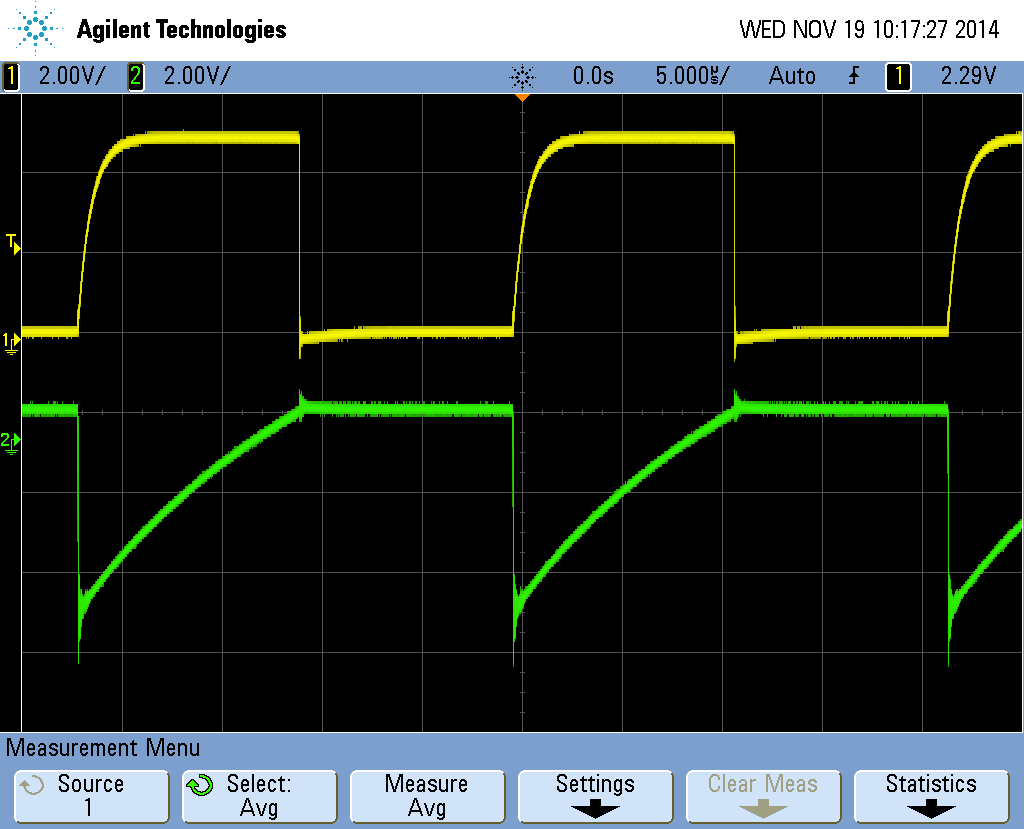
\includegraphics[scale=0.3]{AATC/I1osc.PNG}
\caption{Observations de $V_{C1}$ (en haut) et de $V_{C2}$ (en bas)}
\end{figure}

\noindent Remarque : l'ajout d'un condensateur chimique entre $V_{CC}$ et 0V permet de supprimer du bruit 50Hz qui provient de l'alimentation stabilisée.

\subsubsection*{Simulation à l'aide de PSPICE}

\begin{itemize}
\item Dans un premier temps, l'oscillateur ne démarre pas. En effet, notre étude supposait en condition initiale un état avec un transistor saturé et l'autre bloqué. En réalité, c'est du bruit ou l'imperfection des valeurs des composants qui permet de faire basculer le système dans l'un ou l'autre des états lors de la mise sous tension. La simulation ne prend pas cela en compte, il faut donc préciser une condition initiale sur une des grandeurs (par exemple $V_{B1} = 0$) pour faire démarrer l'oscillateur.
\newpage

\item On reprend la simulation et on affiche les tensions $V_{B1},V_{B2},V_{C1}$ et $V_{C2}$.
\begin{figure}[h!]
\centering
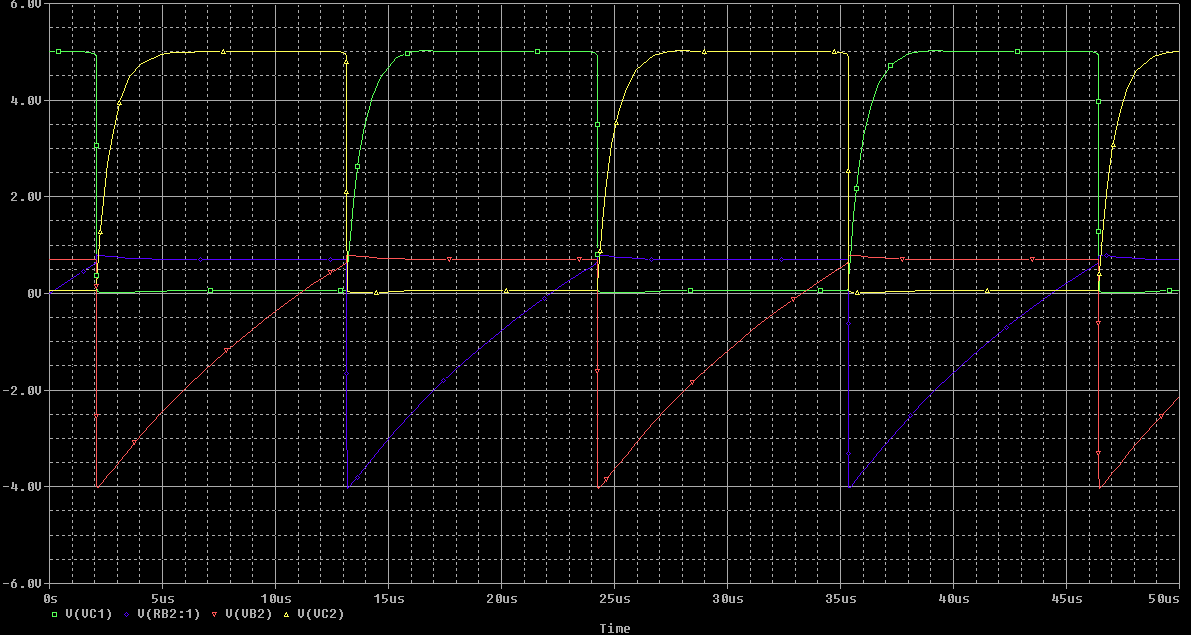
\includegraphics[scale=0.3]{AATC/I1sim4.PNG}
\caption{Tensions $V_{B1},V_{B2},V_{C1}$ et $V_{C2}$ simulées}
\end{figure}

Plus particulièrement, on s'intéresse aux tensions $V_{B1}$ et $V_{C1}$ observées précédemment sur le montage réel.
\begin{figure}[h!]
\centering
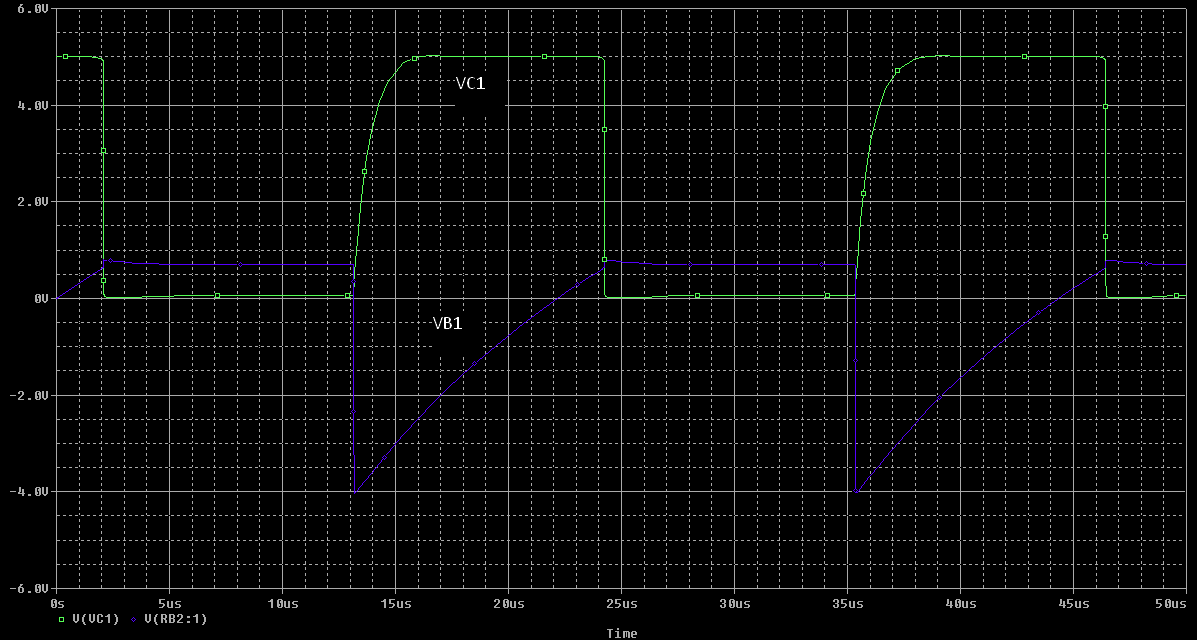
\includegraphics[scale=0.3]{AATC/I1sim.PNG}
\caption{Tensions $V_{B1}$ et $V_{C1}$ simulées}
\end{figure}

Pour mesurer le temps de montée de $V_{C1}$ à 90$\%$, c'est-à-dire à 4,5V puisque $V_{C1}$ varie entre 0V et 5V, on utilise le curseur du logiciel. Le temps de montée est de 1,13$\mu s$.

Le logiciel propose une analyse mathématique des signaux simulés et on peut notamment en extraire la fréquence. On trouve $f=45$kHz.

\subsection*{Retour à la maquette}

\item On se propose de déterminer le temps de montée et la fréquence du signal observé $V_{C1}$. On utilise les fonctions Mesures et Curseurs de l'oscilloscope.

\newpage
\begin{figure}[h!]
\centering
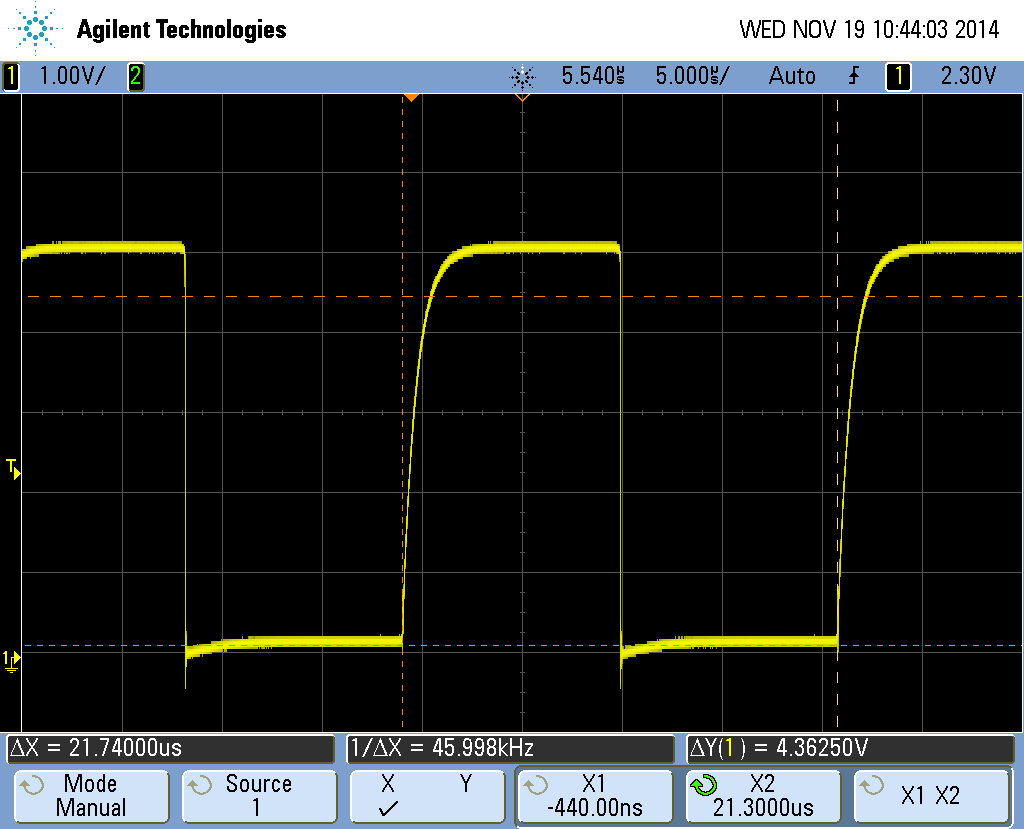
\includegraphics[scale=0.3]{AATC/I1oscfreq.PNG}
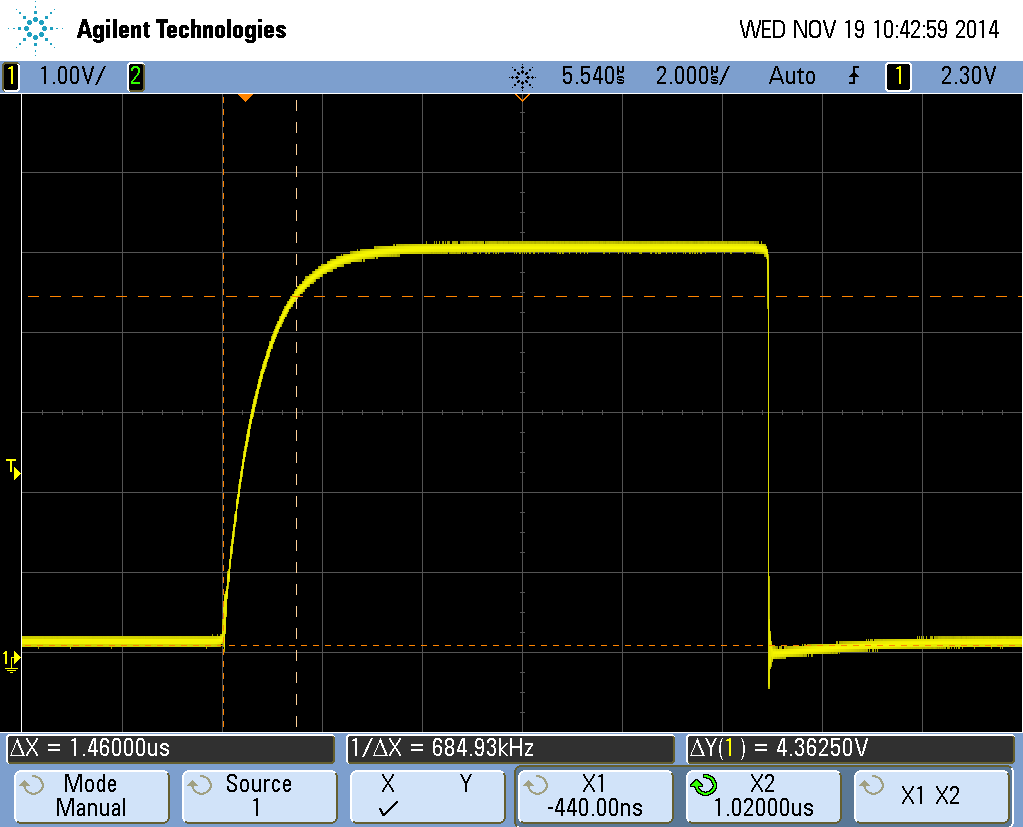
\includegraphics[scale=0.3]{AATC/I1osc90.PNG}
\caption{Détermination de la fréquence et du temps de montée de $V_{C1}$ sur le montage}
\end{figure}

On a donc un temps de montée de $1,46\mu s$ et une fréquence de 46 $kHz$. Ces valeurs sont assez proches de celles obtenues par simulation. La précision des mesures et une éventuelle dispersion de la valeur des composants peuvent expliquer de faibles écarts.

En conclusion, la modélisation réalisée est assez fidèle au montage réel.
\end{itemize}

\newpage
\subsection{L'oscillateur d'Abraham et Bloch avec circuits de mise en forme}
À l'aide du logiciel DSPICE, on relève les formes d'onde de $V_{B1}, V_{B2}, V_{C1}$ et $V_{C2}$ du montage avec circuits de mise en forme.
\begin{figure}[h!]
\centering
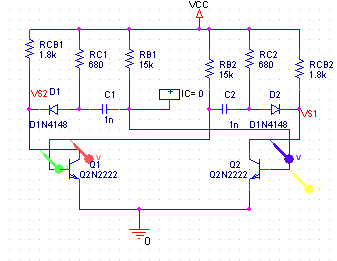
\includegraphics[scale=0.8]{AATC/I2sim.PNG}
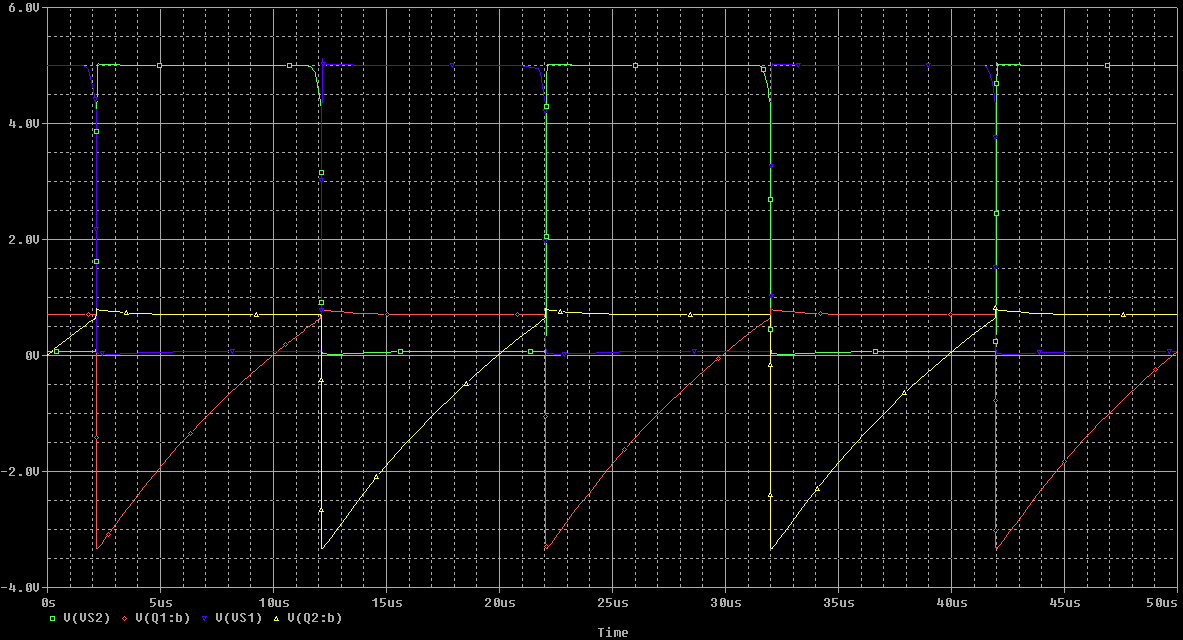
\includegraphics[scale=0.3]{AATC/I2simfreq.PNG}
\caption{Oscillateur d'Abraham et Bloch avec circuits de mise en forme}
\end{figure}

Par rapport au montage précédent, les tensions $V_{C2}$ et $V_{C2}$, qui évoluaient selon la charge d'un condensateur, ont davantage la forme d'un créneau d'amplitude 5V et de valeur moyenne 2,5V.

La fréquence d'oscillation, de 45kHz, est inchangée.

\subsection{L'oscillateur contrôlé en tension}

On utilise la "simulation paramétrique" pour effectuer plusieurs simulation où on fait varier le paramètre $E$, tension d'entrée du VCO.

On peut, à l'aide du menu de fonctions mathématiques, tracer alors la fréquence d'oscillation en fonction de $E$.\\

La pente de la caractéristique est de -21 kHz/V, donc en valeur absolue le gain du VCO est $|K_3|$ = 21 kHz/V.
\begin{figure}[h!]
\centering
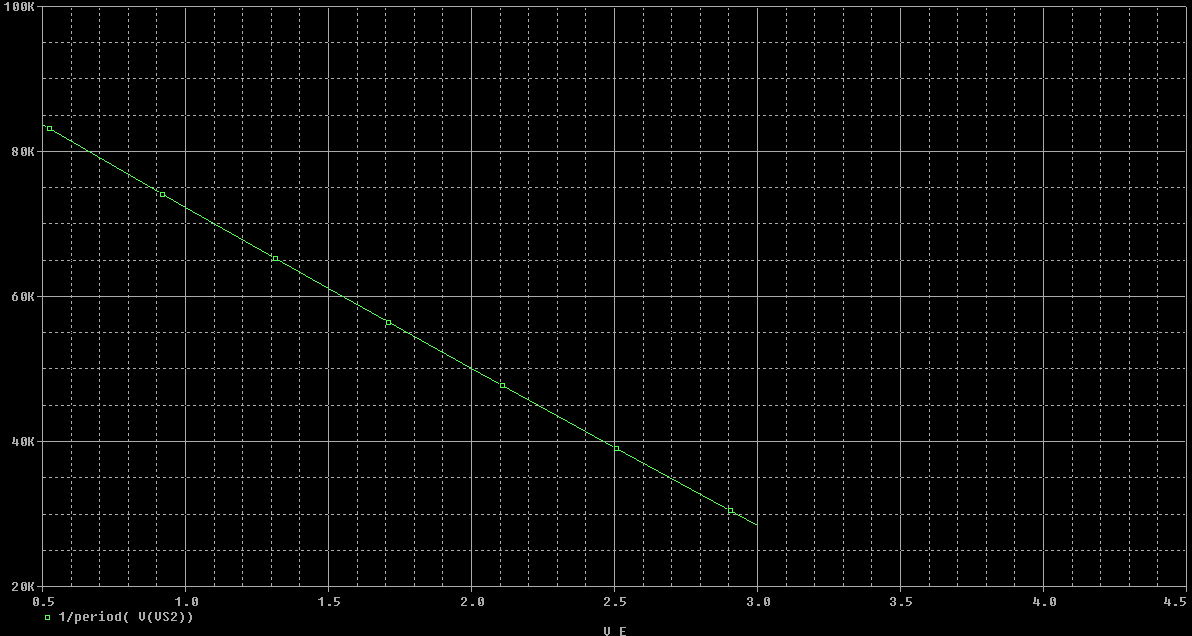
\includegraphics[scale=0.3]{AATC/I3f(E).PNG}
\caption{Caractéristique  fréquence / tension du VCO (simulation)}
\end{figure}

\newpage
\textit{Utilisation de la maquette}\\

En appliquant une tension constante (alimentation stabilisée) à l'entrée du VCO, on observe pour $V_{C1}$ et $V_{B1}$ :
\begin{figure}[h!]
\centering
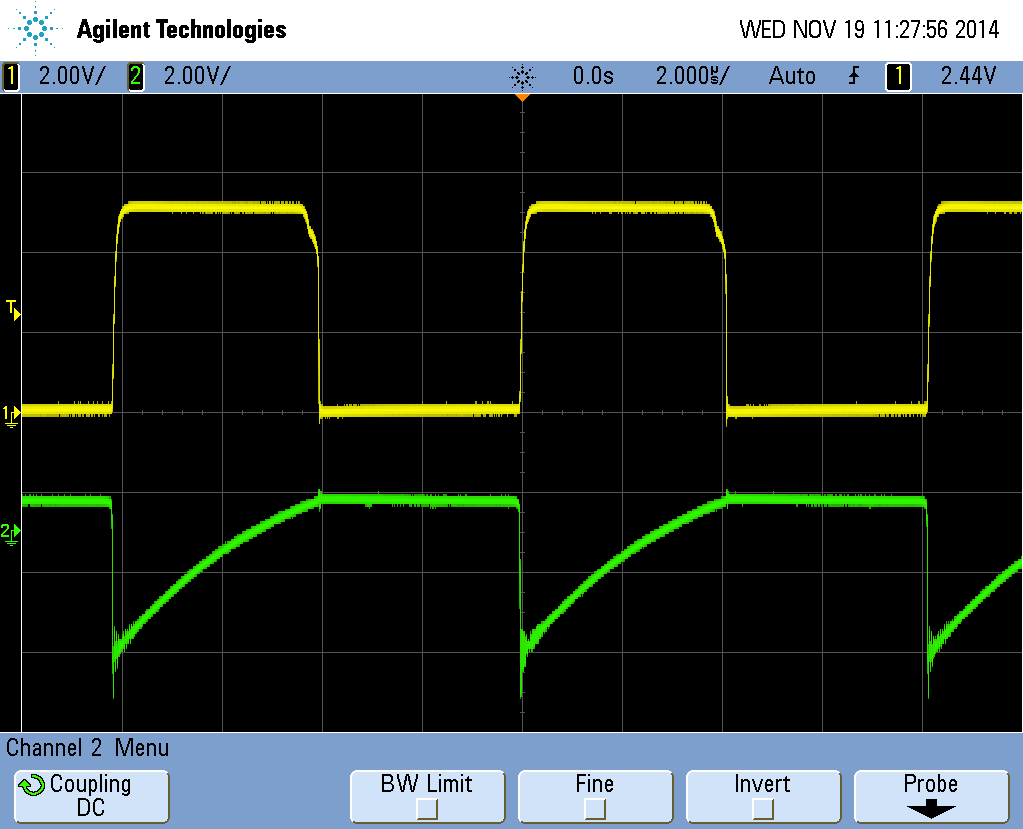
\includegraphics[scale=0.3]{AATC/I3maq.PNG}
\caption{Allure de $V_{C1}$ et $V_{B1}$ observées sur la maquette}
\end{figure}

On obtient bien des créneaux d'amplitude 5V, et de valeur moyenne 2,5V.\\

\newpage
On relève expérimentalement la caractéristique fréquence / tension :

\begin{figure}[h!]
\centering
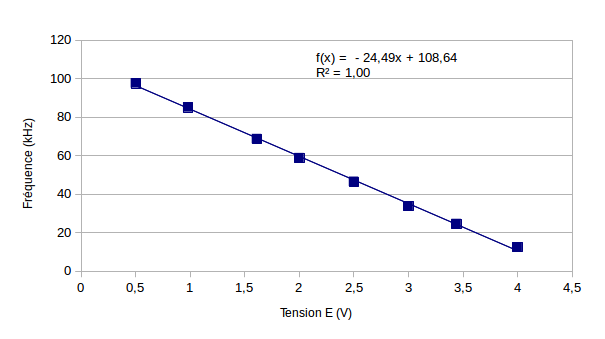
\includegraphics[scale=0.6]{AATC/carac.png}
\caption{Caractéristique expérimentale fréquence / tension du VCO}
\end{figure}

La sensibilité du VCO est donc en valeur absolue de 24,5kHz/V. Cette sensibilité et du même ordre de grandeur que celle attendue dans la préparation et la simulation. L'écart peut se justifier par les défauts physiques induits par les composants.\\

La fréquence $f_m$ correspondant à la moitié de la tension d'alimentation est 46.5kHz.

\newpage
\section{Étude du comparateur de phase OU EXCLUSIF}
On se propose de vérifier le bon fonctionnement du circuit 74HC86 (OU EXCLUSIF) implanté sur la maquette.

On utilise un GBF à deux sorties pour générer des signaux TTL déphasés et on observe la sortie du OU EXCLUSIF pour des signaux déphasés de 90 puis 180 degrés.

\begin{figure}[h!]
\centering
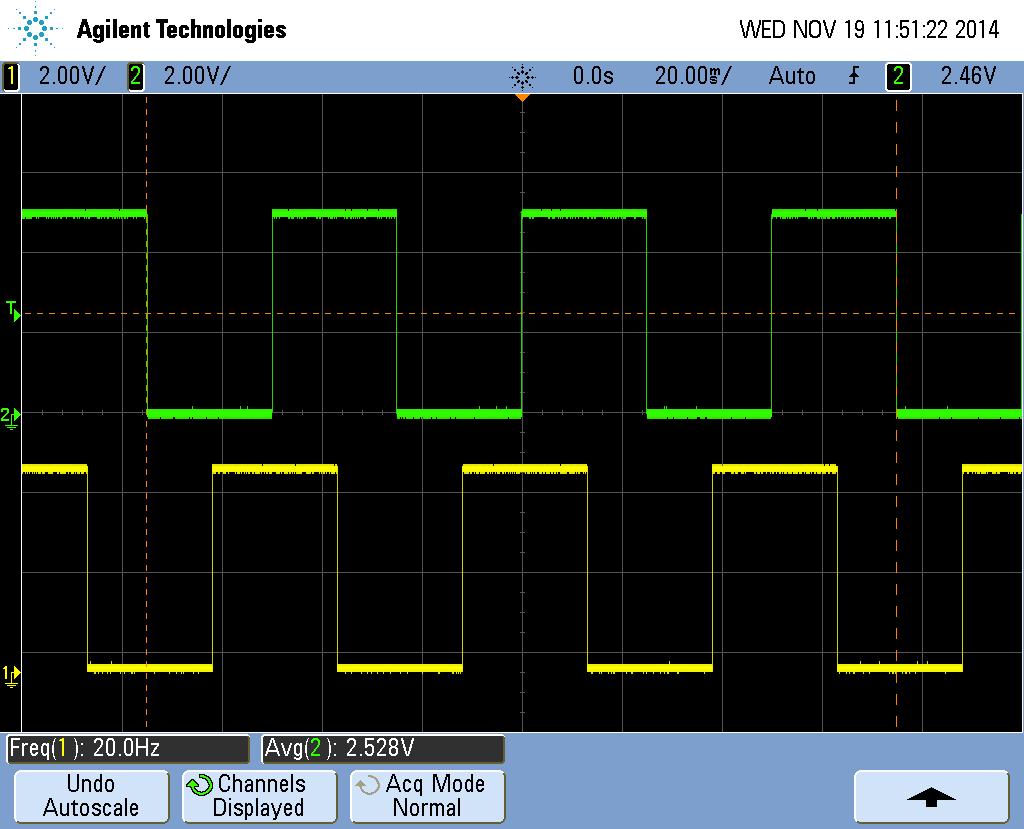
\includegraphics[scale=0.2]{AATC/II90.PNG}
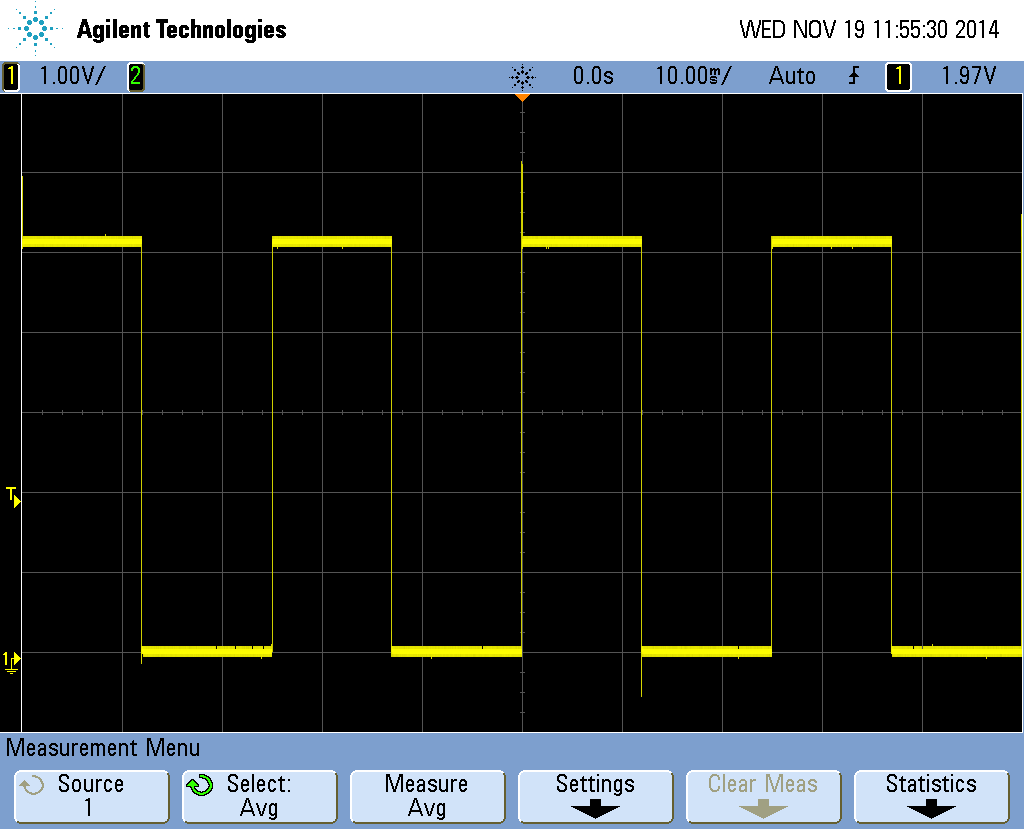
\includegraphics[scale=0.2]{AATC/II90XOR.PNG}
\caption{Entrées déphasées de 90 degrés et sorties du OU EXCLUSIF}
\end{figure}

\begin{figure}[h!]
\centering
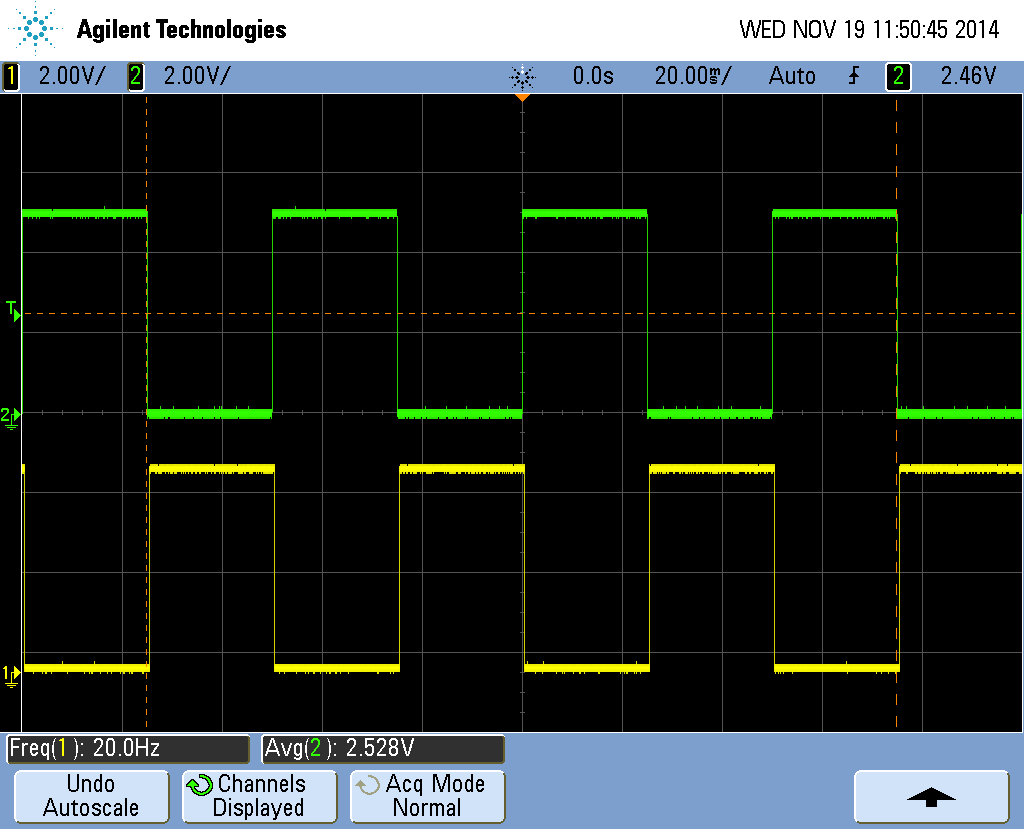
\includegraphics[scale=0.2]{AATC/II180.PNG}
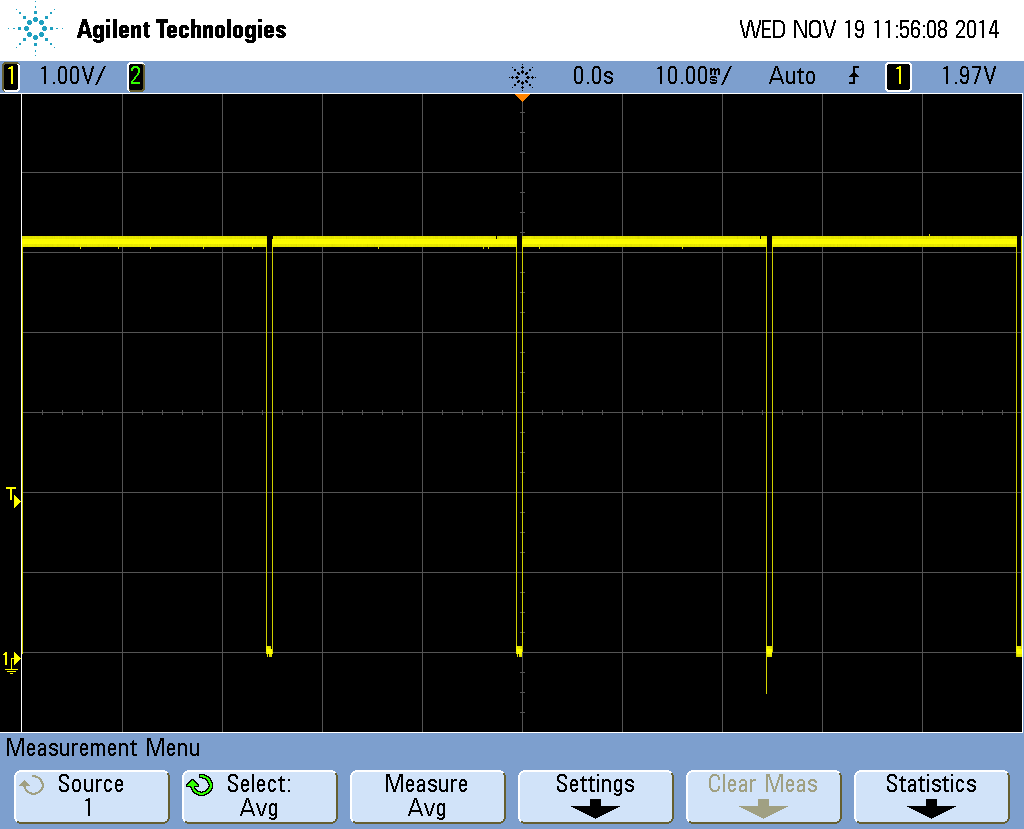
\includegraphics[scale=0.2]{AATC/II180XOR.PNG}
\caption{Entrées déphasées de 180 degrés et sorties du OU EXCLUSIF}
\end{figure}

On a bien le comportement attendu du OU EXCLUSIF.\\

On utilise ensuite la fonction "Mesure / Moyenne" de l'oscilloscope pour tracer la caractéristique valeur moyenne / déphasage entre les entrées.\\

\noindent Il faut afficher un nombre suffisant de périodes à l'écran de l'oscilloscope pour que le résultat de la moyenne soit correct.

\begin{figure}[h!]
\centering
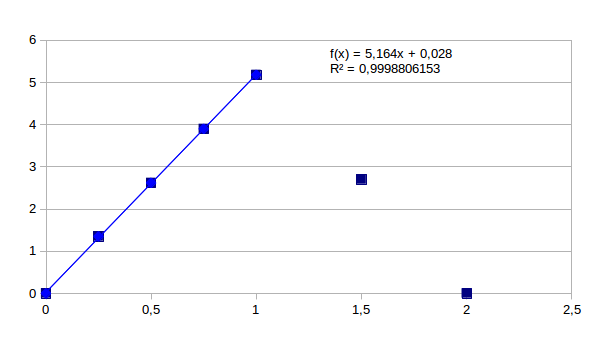
\includegraphics[scale=0.8]{AATC/xor.png}
\caption{Valeur moyenne du signal de sortie du XOR en fonction de $\phi/\pi$, ($\phi$ déphasage entre les entrées)}
\end{figure}

La valeur de $K_1$ correspond à la pente de la caractéristique, donc en valeur absolue, $|K_1| \approx \frac{5,1}{\pi}$ V/rad.s

Cette valeur est très proche de celle donnée dans la préparation.

\newpage
\section{Boucle à verrouillage de phase}

\subsection{Étude de l'asservissement en fréquence}

On réalise le montage avec la fréquence de coupure du passe-bas $f_C = 5$ kHz.

\begin{figure}[h!]
\centering
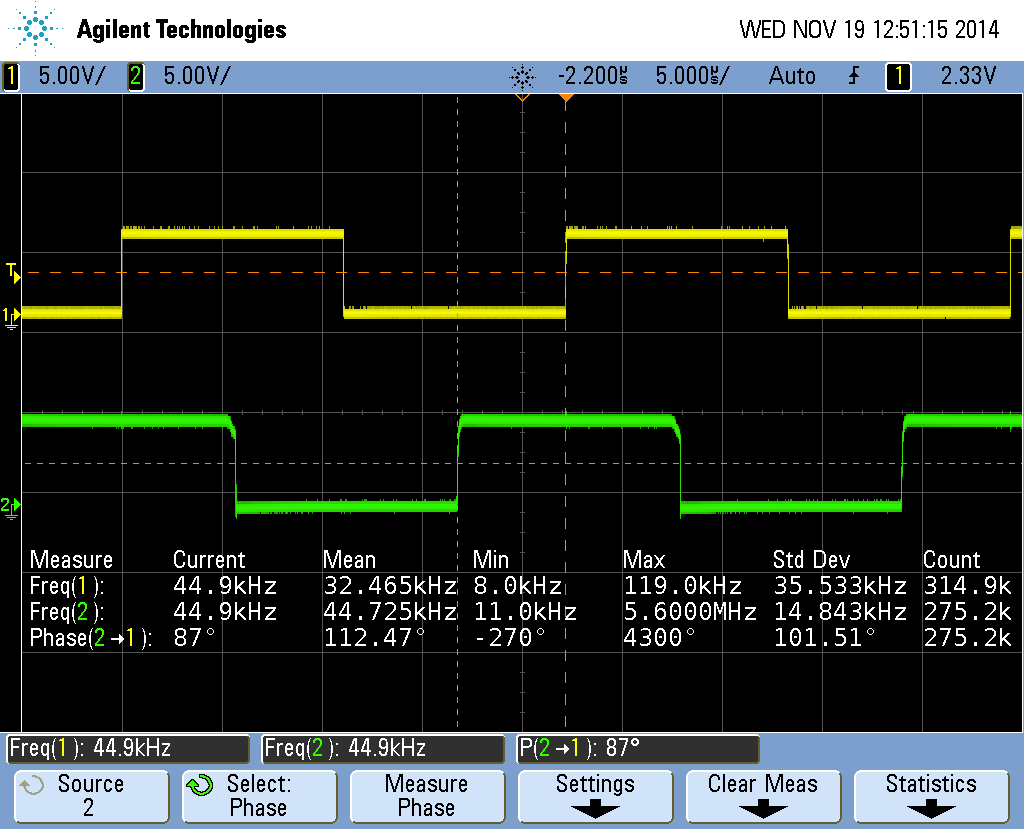
\includegraphics[scale=0.3]{AATC/III145k.png}
\caption{Boucle accrochée pour $f \approx f_m$ (45kHz)}
\end{figure}

\begin{multicols}{2}
Plage de verrouillage :
\[ [f_{Vmin} , f_{Vmax} ] = [15,6 kHz,107kHz ]\]
Plage de capture :
\[ [f_{Cmin} , f_{Cmax} ] = [25,4 kHz,61kHz ]\]
\end{multicols}

On a bien  $ [f_{Cmin} , f_{Cmax} ] \subset [f_{Vmin} , f_{Vmax} ]$.

La largeur de la plage de capture correspond à 36 kHz. En toute rigueur, celle-ci devrait être égale à $2f_c$. Cependant, notre filtre passe-bas n'est pas idéal, et même si $|f-f_0| > f_c$, l'atténuation du filtre n'est pas suffisante pour empêcher l'accrochage de la boucle.

\subsection{Influence du filtre}

On change la fréquence de coupure du filtre $f_c =$ 1kHz.
\begin{multicols}{2}
Plage de verrouillage :
\[ [f_{Vmin} , f_{Vmax} ] = [10 kHz,104kHz ]\]
Plage de capture :
\[ [f_{Cmin} , f_{Cmax} ] = [36 kHz,50kHz ]\]
\end{multicols}

La plage de verrouillage ne change pas. En revanche, la plage de capture a été resserrée.

Nous n'avons pas eu le temps de finir l'étude de la relation entre largeur de la plage de capture et fréquence de coupure du passe-bas.
\end{document}
